%%%%%%%%%%%%%%%%%%don't forget if needed %%%%%%%%%%%%%%%%%%%%%
%\section[toc version]{title version%
%              \sectionmark{head version}}
%\sectionmark{head version}
%%%%%%%%%%%%%%%%%%%%%%%%%%%%%%%%%%%%%%%%%%%%%%%%%%%%%%%%%%%%%%
\def\titcourt{Numerical simulation of 3D configurations using domain decomposition method}
\def\titlong{Numerical simulation of 3D configurations using domain decomposition method}
%%%%%%%%%%%%%%%%%%%%%%%%%%%%%%%%%%%%%%%%%%%%%%%%%%%%%%%%%%%%%%%%
\chapter[\titlong]{\titlong%
              \chaptermark{\titcourt}}
\chaptermark{\titcourt}
\label{chap-3D-SIMULATION}
%%%%%%%%%%%%%%%%%%%%%%%%%%%%%%%%%%%%%%%%%%%%%%%%%%%%%%%%%%%%%%%%
%%%%%%%%%%%%%%%%%%%%%%%%%%%%%%%%%%%%%%%%%%%%%%%%%%%%%%%%%%%%%%%%

Having extensively validated and analysed 2D  melting and solidification configurations for phase-change materials in the previous chapters, we now perform parallel computing of three-dimensional liquid-solid phase-change systems involving natural convection.
We use the recent library \texttt{ffddm} that makes available in FreeFem++ state-of-the-art scalable Schwarz domain decomposition methods (DDM).
Our motivation to expand our numerical model to 3D configuration is first motivated by the lack of publications in the literature for accurate 3D simulations of phase-change materials.
%Also, since publications related to three-dimensional simulation of phase-change material is not abundant in the literature, we expand our numerical model to 3D configuration.
Also, experimental investigations against which we have validated our numerical method involve three-dimensional effects that we have assumed to be neglected in our comparisons.
The latter assumption is however not valid for high $\Ray$ numbers.

The main feature of our numerical approach is the use of 3D adaptive mesh, performed using \textit{mmg3d} library.
\textit{Mmg3d} is a 3D remeshing software developed by \cite{dobrzynski:hal-00681813}, which allows to remesh an initial mesh made of tetrahedra.
The metrics for the mesh adaptation are computed using \textit{mshmet} library, which computes anisotropic metric based on solution variations.
Since the mesh adaptivity procedure is done through a sequential algorithm, we compute the metrics with respect to the coarse mesh, then finer local meshes are then generated in parallel during the mesh decomposition step in order to reach the desired level of refinement for the subdomains.
We use \textit{Metis} library to split the domain into subdomains.
The number of layers of mesh elements in the overlap region between subdomains is set to $2$ for all subsequent simulations.
This chapter is part of the paper [G. Sadaka, A. Rakotondrandisa, F. Luddens, C. Lothod�, P-H. Tournier, I. Danaila, \textit{Parallel finite-element codes for the simulation of solid-liquid phase-change systems with natural convection}, to be submitted to CPC, 2019].

For three-dimensional applications, direct solvers used in the frame of 2D problems are not appropriate and iterative methods must be employed since memory requirements for \textit{LU} decomposition would rapidly exceed the capacity of available computers.
The linear system of equations resulting from the Newton linearisation are thus solved using parallel \textit{GMRES} Krylov method.
Since it is well known that iterative methods can suffer from convergence problems, we adapt the number of subdomain in such a way that each processor could handle $1,000$ tetrahedra.
The Optimized Restricted Additive Schwarz (ORAS) preconditioned \textit{GMRES} solver proved to be extremely efficient since an order of 30 iterations were necessary to get a residual norm of $10^{-9}$ for each Newton iteration.
We note that in all numerical simulations, a quadratic ($\PP_2$) discretization of $\theta$ was used.

The remainder of this chapter is as follows.
In Sec. \ref{sec: natconv-air-3D}, we validate the 3D natural convection of air inside differentially heated cube against numerical benchmark by \cite{Wakashima-2004}.
We also compare the solutions obtained by the parallel computation with the solution obtained using sequential algorithms.
Then, the natural convection of water is investigated in Sec. \ref{sec-3D-water-convec}. %to illustrates the capability of our method to deal with non-linear body force $f_B$ and to capture accurately interfaces, mainly the density inversion.
Finally, the lateral melting of n-octadecane PCM inside 3D enclosure is addressed.

\section{Numerical simulation of the natural convection of air in 3D configurations}\label{sec: natconv-air-3D}
 Following the same line of argument that was outlined in Chapters. \ref{chap-NATCONV} and \ref{chap-MELTING}, we start by presenting the natural convection of air, that involves linear description of the buoyancy force $f_B$, and include gradually additional non-linearities.
The well-known thermally driven cavity is addressed first in Sec. \ref{subsec-3D-natconv-air}. %and the problem is then complicated by incorporating a heated cube in the center of the domain in Sec. \ref{sub-OBSTACLE-3D}.
The physical parameters are the same than used in the 2D simulations ($\Prd = 0.71$) and we investigate three Rayleigh numbers: $\Ray=10^4$, $\Ray=10^5$, and $\Ray=10^6$. 
The walls are rigid and impermeable. The vertical walls at $x=0$ and $x=1$ are isothermal and have different temperatures $T_h = 0$ and $T_c = 1$ respectively. The remaining walls are considered adiabatic. 
The fluid is initially at rest and the temperature is linearly distributed from the cold to the hot walls.
We solve the steady Eq. \ref{eq-weak-steady} by increasing smoothly the parameter $\alpha$ before the Boussinesq term (which can be assimilated to a Rayleigh continuation step) with a maximum of $6$ steps for $\Ray = 10^6$.

\begin{figure}
\begin{minipage}{\linewidth}
\begin{center}
 {\includegraphics[width=.95\textwidth]{\figpath/Fig_cap_natconv/Validation_3D_seq_T1}}
\end{center}
\end{minipage}
\caption{3D differentially heated cavity. Temperature contours at the mid-plane of ($y=0.5$); comparison with the results of \cite{Wakashima-2004} (left images). }
\label{fig-3DT} 
\end{figure}
We first compare the current simulation with the numerical data of \cite{Wakashima-2004}, who have used a forth order finite difference method, with a vorticity-stream function formulation with different uniform meshes of  $120 \times 120 \times 120 \times 10$ grid nodes.
Our results were obtained using uniform grids of $ 40 \times 40 \times 40$.
Since the converged flow pattern and temperature distributions are symmetrical with respect to the center of the cavity for the investigated Rayleigh number,
we display in 
Fig. \ref{fig-3DT} the temperature field at the mid section ($y = 0.5$), for each of the three Rayleigh numbers $\Ray = 10^4$ (top), $\Ray = 10^5$ (middle), $\Ray = 10^6$(bottom).  
On the left we display the numerical results of \cite{Wakashima-2004} and on the right the present simulation.
The comparison with the benchmark solution exhibits a fairly good agreement with the considered test case.
The higher the Rayleigh number, the finner the thermal boundary layer thickness in the vicinity of the vertical walls.
One can also notice the stagnant fluid with stratified temperature in the center of the domain in both numerical solutions.

More accurate comparison is addressed in Tab. \ref{tab-3D-locU} between the present simulation and numerical data from the literature.
We assess the maximum velocity values and their corresponding location with benchmark solution of \cite{Wakashima-2004} and numerical results of \cite{Raluca2013}.
The solutions show a good convergence on a mesh $3$ times coarser than the one proposed by  \cite{Wakashima-2004} and an excellent agreement is found for all values of the Rayleigh number.
For $\Ray = 10^4$ the current simulation shows a relative difference of $0.15 \%$ for $u_{max}$ and $0.28 \%$ for $v_{max}$ with the latter.
Larger differences of $6.55 \%$ is found with those obtained by \cite{Raluca2013}, since their results are smaller than the considered benchmark.
However, for $\Ray = 10^5$ and $10^6$ the results are in good agreement.


\begin{table}
   \begin{center}
      \begin{tabular}{*{3}{cl}}
           & $u_{max}$ ($y$) & $v_{max} ($x$)$ \\ \toprule
           $\Ray = 10^4$ & $0.198094$ ($0.826772$) & $0.220973$ ($0.11811$) \\ 
           \cite{Wakashima-2004} & $0.1984$ ($0.8250$) & $0.2216$ ($0.1177$) \\
           \cite{Raluca2013} & $0.1859$ ($0.8230$) & $0.2234$ ($0.1172$) \\ \hline
           
           $\Ray = 10^5$ & $0.140367$ ($0.850394$) & $0.245454$ ($0.0629921$) \\ 
           \cite{Wakashima-2004} & $0.1416$ ($0.8500$) & $0.2464$ ($0.0677$) \\
           \cite{Raluca2013} & $0.1461$ ($0.8540$) & $0.2459$ ($0.0703$) \\ \hline
           
           $\Ray = 10^6$ & $0.0809247$ ($0.858268$) & $0.257719$ ($0.0393701$) \\ 
           \cite{Wakashima-2004} & $0.08111$ ($0.8603$) & $0.2583$ ($0.0323$) \\ 
           \cite{Raluca2013} & $0.0830$ ($0.8550$) & $0.2553$ ($0.03905$) \\ \bottomrule
          
           
               \end{tabular}
   \end{center}
   \caption{3D differentially heated cavity. Comparison with benchmark solutions for $\Ray = 10^4$, $\Ray = 10^5$, $\Ray = 10^6$.}
   \label{tab-3D-locU}
\end{table}

Further comparison of the the parallel solver with the sequential algorithm is offered in Tab. \ref{tab-T1} for all cases. 
\begin{table}
	\begin{center}
		\begin{tabular}{|*{6}{c|}}
			\hline
			 $\Ray$ & \em{nb proc }                  & $||u||_{2}$                        & $||u||_{\infty}$                & $||T||_{2}$              & $||T||_{\infty}$\\ \hline \hline
			\multirow{4}{*}{$10^4$} & 28 & $1.12496 \cdot 10^{-6}$ & $3.1 \cdot 10^{-6}$ & $ 3.09966 \cdot 10^{-6} $ & $7 \cdot 10^{-6}$ \\% \hline
			\cline{2-6}
			& 42 & $1.53698 \cdot 10^{-6}$ & $5.1 \cdot 10^{-6}$ & $ 3.23352 \cdot 10^{-6} $ & $8 \cdot 10^{-6}$ \\ \cline{2-6} %\hline 
			& 56 & $1.55576 \cdot 10^{-6}$ & $5.1 \cdot 10^{-6}$ & $ 3.4342 \cdot 10^{-6} $ & $8 \cdot 10^{-6}$  \\ \cline{2-6} %\hline
			& 70 & $1.25622 \cdot 10^{-6}$ & $3.6 \cdot 10^{-6}$ & $ 3.56048 \cdot 10^{-6} $ & $8 \cdot 10^{-6}$ \\ \hline \hline
			\multirow{4}{*}{$10^5$} & 28 & $1.73254 \cdot 10^{-6}$ & $6.1 \cdot 10^{-6}$ & $ 2.40467 \cdot 10^{-6} $ & $7 \cdot 10^{-6}$ \\% \hline
			\cline{2-6}
			& 42 & $2.84973 \cdot 10^{-6}$ & $7.78 \cdot 10^{-6}$ & $ 3.53003 \cdot 10^{-6} $ & $9 \cdot 10^{-6}$ \\ \cline{2-6} %\hline 
			& 56 & $3.00832 \cdot 10^{-6}$ & $7.39 \cdot 10^{-6}$ & $ 4.17769 \cdot 10^{-6} $ & $1.1 \cdot 10^{-5}$  \\ \cline{2-6} %\hline
			& 70 & $3.68118 \cdot 10^{-6}$ & $9 \cdot 10^{-6}$ & $ 4.70846 \cdot 10^{-6} $ & $1.2 \cdot 10^{-5}$ \\ \hline \hline
			\multirow{4}{*}{$10^6$} & 28 & $6.61804 \cdot 10^{-6}$ & $1.826 \cdot 10^{-5}$ & $ 3.46504\cdot 10^{-6} $ & $1.1 \cdot 10^{-5}$ \\% \hline
			\cline{2-6}
			& 42 & $5.93966 \cdot 10^{-6}$ & $1.5 \cdot 10^{-5}$ & $ 3.98082 \cdot 10^{-6} $ & $1.2 \cdot 10^{-5}$ \\ \cline{2-6} %\hline 
			& 56 & $7.05144 \cdot 10^{-6}$ & $1.9247 \cdot 10^{-5}$ & $ 5.0044 \cdot 10^{-6} $ & $2 \cdot 10^{-5}$  \\ \cline{2-6} %\hline
			& 70 & $6.02152 \cdot 10^{-6}$ & $1.68 \cdot 10^{-5}$ & $ 4.50094 \cdot 10^{-6} $ & $1.8 \cdot 10^{-5}$ \\ \hline
		\end{tabular}
	\end{center}
	\caption {3D differentially heated cavity. Comparison between sequential and ffddm algorithm for uniform grids of $40 \times 40 \times 40$ }
	\label{tab-T1}
\end{table}
We compute $L^2$ and $L^\infty$ norms of the velocity and the temperature.
The number of subdomain varies from $28$ to $70$ for $1.8$ millions of unknown to assess the consistency of our method with the number of subdomains 
The difference between both algorithm is of order of $10^{-6}$
and we do not observe a large variation of the error when the number of subdomains keep increasing.
The comparison with the sequential algorithm was limited to $40 \times 40 \times 40$ grids size since the simulations are highly demanding in CPU time.
The steady state solution required $57$ CPU hours and $3$ runs (restarts) with $120$ Go of memory for the sequential algorithm, for the highest value of the Rayleigh number. 
The computational time is considerably reduced using DDM and 3D simulations becomes affordable  since only $21$ CPU minutes  ($1308.48$ s) were necessary with $70$ processors to achieve the same case with an error of $6.02152 \cdot 10^{-6}$ on $\vec u$ and $ 4.50094 \cdot 10^{-6} $ on $\theta$.


%\subsection{Natural convection in a cube with an inner heated obstacle}\label{sub-OBSTACLE-3D}
%A heated obstacle, at constant temperature $\theta_o = 0.8$, is included in the center of the unit cube as depicted in Fig. \ref{fig-obstacle-Ra1e4}.
%The vertical walls are differentially heated with $\theta_h = 0.5$ and $\theta_c = -0.5$.
%Simulation is performed for $\Ray = 10^6$.
%
%The temperature contours at the mid-plane is displayed in Fig. \ref{fig-obstacle-Ra1e4}b.
%At the investigated Rayleigh number, the heat transfer is completely governed by convection.
%A plume, tilted to the right, towards cold wall could be observed above the hot obstacle.
%The clockwise recirculation of the fluid transport actually the heated air from the hot (center) obstacle to the cold (right) wall.
%When compared to the two-dimensional case, the flow inside the 3D cubic box is obviously more complex, since a spiral movement of the fluid occurs along the walls whereas boundary layer heat transfer takes place in the same region.
%
%We also assess The number of CPU used were chosen to satisfy the criterion degrees of freedom per CPU in the range of $50,000$ to $200,000$.
%
%
%
%
%\begin{table}
%\begin{center}
%\begin{tabular}{|*{7}{c|}}
%
%		\hline
%                $\Ray$ & \em{nbseg} & \em{nb proc }                    & $||u||_{2}$                        & $||u||_{\infty}$                & $||T||_{2}$              & $||T||_{\infty}$\\ \hline \bottomrule
%                \multirow{12}{*}{$10^6$}& \multirow{4}{*}{40} & 28 & $0.000830258$ & $0.0203142$ & $ 0.0017393 $ & $0.034896$ \\ \cline{3-7}
%                & & 42 & $0.000831142$ & $0.0203468$ & $ 0.00175767 $ & $0.034882$ \\ \cline{3-7}
%                & & 56 & $0.00085423$ & $0.0203416$ & $ 0.00181677 $ & $0.034887$ \\ \cline{3-7}
%                & & 70 & $0.00083373$ & $0.0203248$ & $ 0.00175643 $ & $0.03489$ \\ \cline{2-7}
%                & \multirow{4}{*}{60} & 112 & $0.000420192$ & $0.0023909$ & $ 0.000953569 $ & $0.01381$ \\ \cline{3-7}
%                & & 140 & $0.000416573$ & $0.002334$ & $ 0.000947099 $ & $0.013775$ \\ \cline{3-7}
%                & & 168 & $0.000405618$ & $0.002399$ & $ 0.000923159 $ & $0.013755$ \\ \cline{3-7}
%                & & 196 & $0.000412466$ & $0.0024075$ & $ 0.000945884 $ & $0.013725$ \\ \cline{2-7}
%                & \multirow{4}{*}{80} & 224 & $0$ & $0$ & $ 0 $ & $0$ \\ \cline{3-7}
%                & & 238 & $0.000109568$ & $0.0005326$ & $ 0.000215454 $ & $0.000984$ \\ \cline{3-7}
%                & & 252 & $0.000126653$ & $0.0006788$ & $ 0.000215497 $ & $0.001115$ \\ \cline{3-7}
%                & & 266 & $8.37328\cdot10^{-5}$ & $0.00034267$ & $ 0.000167761 $ & $0.000663$ \\  \toprule
%      
%\end{tabular}
%\end{center}
%\caption {3D convection in a cube with an inner heated cube. Comparison with respect to the most resolved solution ({\em nbseg} $= 80$) for $\Ray = 10^6$.}
%\label{tab-T2}
%\end{table}
%
%
%
%
%\begin{figure} [!ht]
%\begin{center}
%\begin{minipage}{\linewidth}
% {\includegraphics[width=0.98\textwidth]{\figpath/Fig_cap_natconv/3D_OBSTACLE_field_2}}
%\end{minipage}
%\end{center}
%\caption{3D convection in a cube with an inner heated cube. Temperature fields for $Ra = 10^6$.}
%\label{fig-obstacle-Ra1e4} 
%\end{figure}
%
%\clearpage
%\newpage
\section{Numerical simulation of the natural convection of water in a cube cavity.} \label{sec-3D-water-convec}

We perform the natural convection of water inside cubic cavity using adaptive mesh in this section.
The dimensionless parameters are the same that used in Chapter \ref{sec: natconv-water} ($\Ray=2.518084\cdot 10^{6}$ and $\Prd=6.99$).
We impose cold dimensionless temperature $\theta_c = 0$ at $x=1$ (right wall), hot temperature $\theta_h = 1$ at $x=0$ (left wall), and a homogeneous Neumann boundary condition at the remaining walls.
Dirichlet boundary condition $\vec u = 0$ is prescribed over the whole $\partial \Omega$.
In view of anomalous thermal variation of water density, we adapt the mesh along $\theta = 0.4$ to capture correctly the flow structure.
The main limitation of 3D simulations of water convection in the literature is indeed the size of the mesh resolution when fixed grid models are used.
As an example, \cite{Giangi-2000} and \cite{Kowalewski-2003}  have investigated a mesh sensitivity analysis, and have concluded that even by using $81^3$ grid points, the variation of the velocity was still significant,
and beyond such mesh resolution, the problem becomes computationally expensive. %, limiting their analysis.
%Hence, using adaptive mesh helps considerably to combine accuracy and efficiency.

The temperature distribution and the corresponding adapted mesh, at the steady state is shown in Figs. \ref{fig-3D_Water_convec}a. 
The blue region denotes the cold water trapped by the abnormal fluid recirculation and the red region the hot fluid triggered by the upper clockwise circulation.
A zoom of the mesh at the mid-plane is also offered in \ref{fig-3D_Water_convec}b.
Smaller tetrahedra are clearly observed close to the wall, where a spiral movement of the fluid occurs along the walls whereas boundary layer heat transfer takes place in the same region, and between the two counter-rotating circulation patterns.
A minimum edge length $h_{min} = 3.33 \cdot 10^{-3}$ is applied along the maximum density variation, and $h_{max} = 0.15$ in the stagnant fluid region.
The combined mesh adaptation strategy and efficient parallel algorithm, reduces considerably the computational time since only $5012.04$ CPU seconds were necessary to perform the steady solution with $500,000$ tetrahedra using $56$ processors, while \cite{michalek2005natural} have spent $3.6  \times 10^5$ CPU seconds to compute the steady solution with $81^3$ fixed grid points.

In many cases, it is justifiable to perform two-dimensional numerical simulations, since it substantially reduces the computational effort and allows many simulations to be achieved in a realistic time.
However, Fig. \ref{fig-3D_Water_convec}b shows that the three-dimensionality of the flow in cube shape cavity affects the shape of the iso-surface $\theta=0.4$.
\cite{Giangi-2000} have assessed the effect of three-dimensionality in both convection and freezing of water and they have noted that only the flow in the symmetry plane can be treated as two-dimensional.
The no-slip velocity and the adiabatic thermal boundary conditions at the side walls enhance the three-dimensional effect near the walls.
Furthermore, even though the temperature profiles match well for both $2-$ and $3-$D solutions, at the central cross-section of the cavity, the authors have noted that serious differences between two and three-dimensional velocity profiles are always present at some points.

In Figs. \ref{fig-3D_Water_convec}d-f, we plot the velocity profiles along the vertical line passing through the velocity saddle point, where normal and abnormal convection streams collide in the vicinity of the cold wall.
For the $\vec e_z$ component $W$ of the velocity profile along $z-$ direction at $x = 0.93$, we could compare both two and three-dimensional simulations with available $3-$D simulation of \cite{Kowalewski-2003}.
Triangular symbol denotes the reference solution, obtained with 3D finite difference code using vorticity-vector potential formulation of the Navier-Stokes and energy equations.
$3-$D (red solid line) profile agree well with the benchmark solution with a maximum differences of $3 \%$.
The $2-$D (green dashed line) solution exhibits higher discrepancies in the vicinity of the anomalous density variation where the three-dimensional effect is maximum.
However, as noted by \cite{Giangi-2000} in their experimental observations, larger differences between $2-$D and $3-$D solutions could be observed at $x=0.1$ and $x=0.5$.
Panels (e) and (f) exhibit discrepancies greater than $10 \%$ between both solutions in accordance with the foregoing observation.

\begin{figure}
\begin{center}
\begin{minipage}{\linewidth}
 {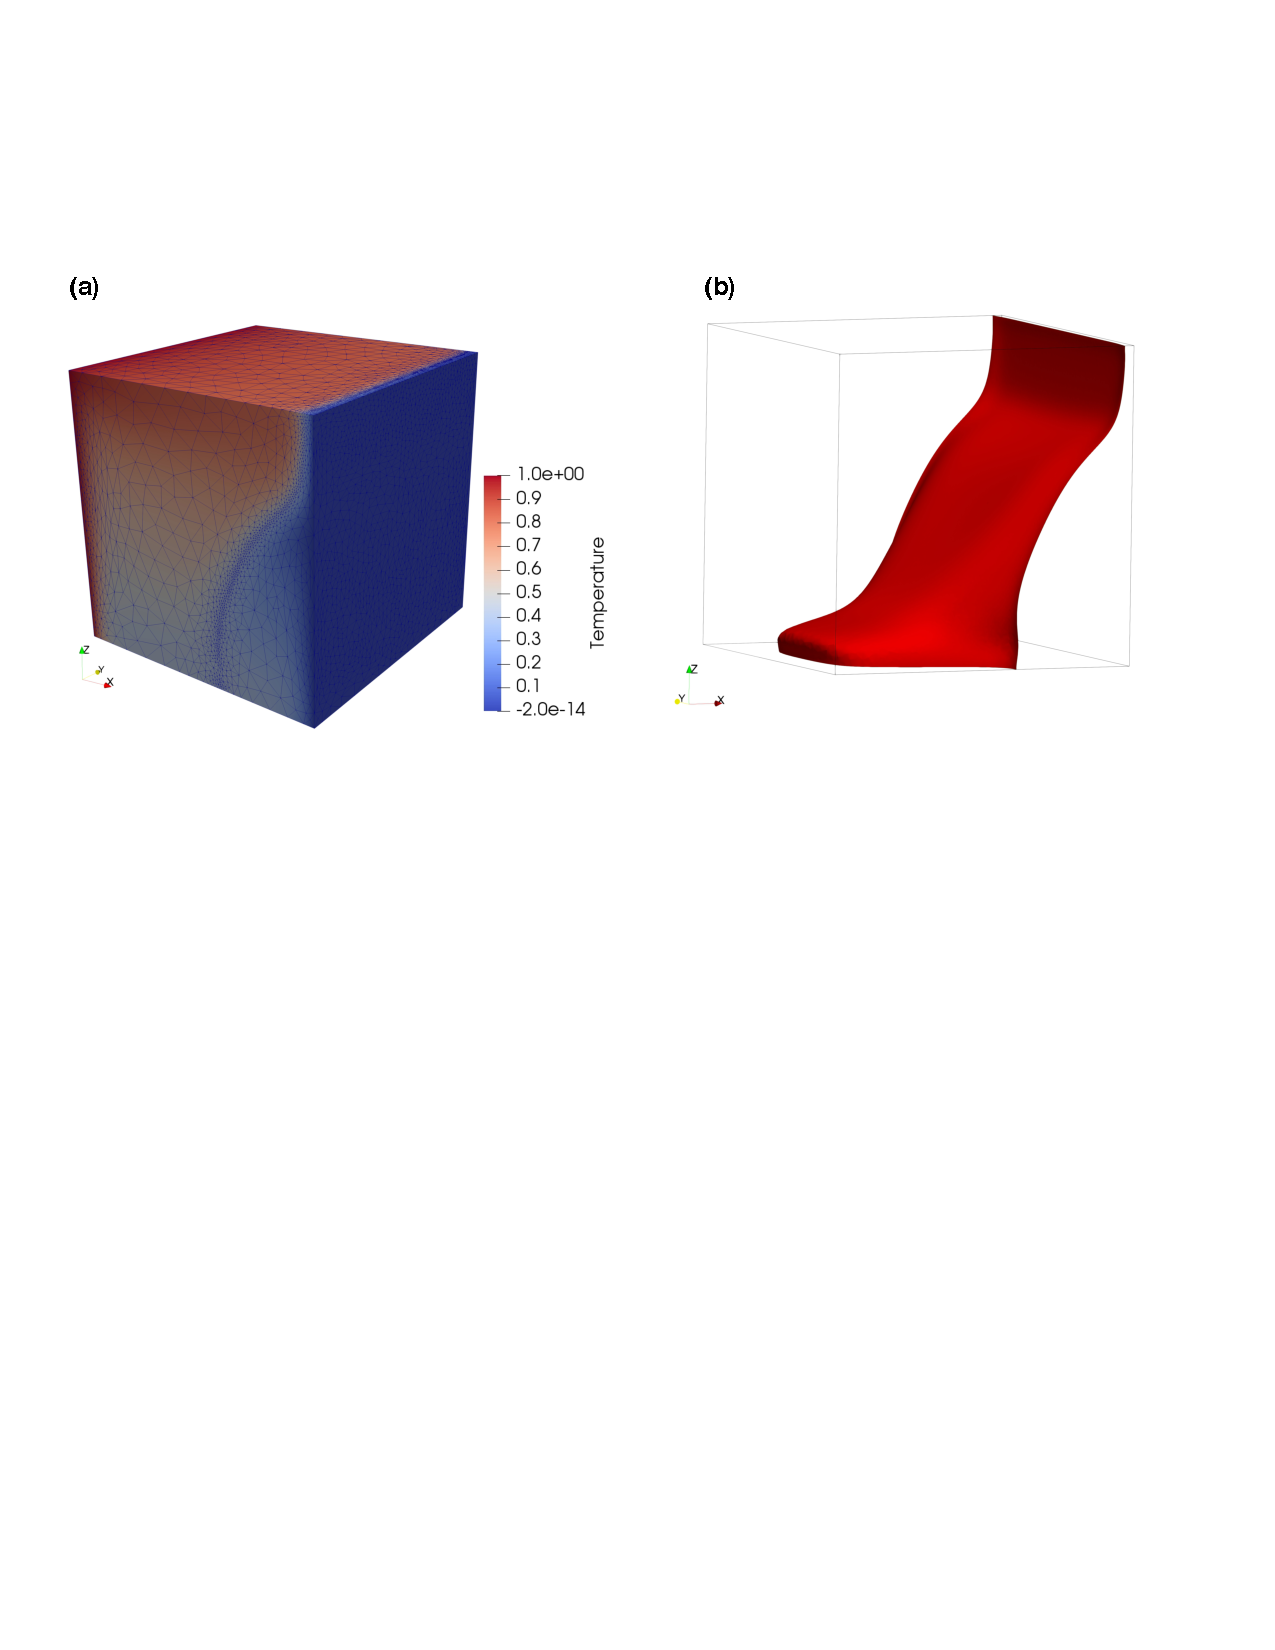
\includegraphics[width=0.9\textwidth]{\figpath/Fig_cap_natconv/3D_WaterConvec}}
 {\includegraphics[width=0.9\textwidth]{\figpath/Fig_cap_natconv/3D_WaterConvec_2}}
\end{minipage}
\end{center}
\caption{3D convection of water in a cube with an inner heated cube. (a) Temperature distribution and adapted mesh. (b) Zoom of the 3D adapted mesh at mid-plane. (c) Iso-surface $\theta = \theta_m$. (d) Comparison of the profile of the vertical velocity along $z-$direction, at the midplane ($y=0.5$) and $x=0.93$ with numerical benchmark by  \cite{Kowalewski-1999}.}
\label{fig-3D_Water_convec} 
\end{figure}

\section{3D numerical simulations of melting with convection}
